% CS 217A/B, Winter/Spring 2017
% Professor Lixia Zhang
% Project Final Report

\documentclass{sig-alternate}

% General packages and setup
\PassOptionsToPackage{hyphens}{url}\usepackage{hyperref}  % For embedding clickable links to citations
\paperheight=11in
\renewcommand\_{\textunderscore\allowbreak}  % Allows line breaks on words with underscores

% Begin packages/setup for timeline
%\usepackage[utf8]{inputenc}
%\usepackage[TS1,T1]{fontenc}
%\usepackage{fourier, heuristica}
%\usepackage{array, booktabs}
%\usepackage{graphicx}
%\usepackage[x11names]{xcolor}
%\usepackage{colortbl}
%\usepackage{caption}
%\usepackage{tikz}  % checkmark icon
%\usepackage{wrapfig}
%\usepackage{soul}  % strikethrough
%
%\DeclareCaptionFont{blue}{\color{LightSteelBlue3}}
%\newcommand{\foo}{\color{LightSteelBlue3}\makebox[0pt]{\textbullet}\hskip-0.5pt\vrule width 1pt\hspace{\labelsep}}
%\def\checkmark{\tikz\fill[scale=0.4](0,.35) -- (.25,0) -- (1,.7) -- (.25,.15) -- cycle;}	% Checkmark icon
% End packages/setup for timeline

\begin{document}
	
\title{ndnMouse\\Secure Control Interface for a PC Using a Mobile Device}
\subtitle{CS 217B Project Final Report, Spring 2017}
\numberofauthors{1}
\author{
	Wesley Minner\\
	Computer Science M.S. Student\\
	wesleyminner@gmail.com
}

\date{18 May 2017}
\maketitle

% ==============================================================================
\begin{abstract}
This report outlines the results of my efforts on ndnMouse, my class project for CS 217B, as well as my Master's Capstone project. It is open-sourced on \href{https://github.com/wminner/ndnMouse}{Github} under the GNU public license, and available on the \href{https://play.google.com/store/apps/details?id=edu.ucla.cs.ndnmouse}{Google Play App Store}. The goal of ndnMouse is to securely and efficiently control one or more personal computers via remote mouse movement and rudimentary keyboard commands from your phone, running the communication protocol over Named-Data-Networking~\cite{ndn} (NDN). In order to compare the design and performance benefits of NDN, ndnMouse also supports communication over UDP. Implementation of both protocols resulted in fairly unique server and clients designs. The pros and cons of each will be explored in this report.

Section 1 will review the features and use cases of ndnMouse, with more detail of the command protocol in Section 2. Details on the security features will be given in section 3, with challenges and trade-offs I have overcome listed in section 4. Performance analysis comparing NDN and UDP implementations is in section 5. Finally section 6 explores extensions and future use cases for ndnMouse. Additionally screenshots of the application are in section 7, the Appendix.
\end{abstract}

\keywords{NDN, Mouse, Keyboard, Remote Access, Security}

% ==============================================================================
\section{Feature Overview}
%So far all of my projected libraries and resources have done well to meet my expectations during implementation.  PyAutoGui~\cite{pyautogui} has performed well as an interface to the PC's mouse, and also conveniently provides configurable text dialog popups as seen in Figures \hyperlink{fig:client1}{5} and \hyperlink{fig:client2}{6}, under the Appendix. The two NDN~\cite{ndn} libraries I mentioned in my proposal, jNDN~\cite{jndn} and pyNDN~\cite{ndn-py} have also met all my expectations.  I have had little to no trouble working with the libraries or understanding the API.
%
%As of the now (the end of 5th week), I have functional UDP and NDN client/server applications, both with symmetric encryption support via the user-password.

\section{Protocol}
%My application runs a custom, connectionless protocol (for both UDP and NDN implementations) that passes simple man-readable (when unencrypted) mouse control commands in the form of 48 byte packets (when using security). The protocol is not optimal regarding the encoding of commands. However the man-readable nature of the commands has made debugging considerably easier during development. I may consider re-designing the protocol when I know the entire command set that the app will need to handle.  However at most, I can save 16 bytes off of each packet (lowering the total packet size to 32 bytes). This is due to the requirements of AES~\cite{cipher} cipher block chaining (CBC), which supports key lengths of 128, 192, and 256 bits. I am using a 128 bit (16 byte) key from the hashed user-password, so the total packet length must always be a multiple of 16 bytes. A 16 byte, random, cleartext initialization vector (IV) must also be included in each packet to ensure that two packets with the same cleartext content never encrypt to the same ciphertext. A 16 byte IV and a 16 byte message results in a minimum packet size of 32 bytes. I may consider using another style of AES encryption (like electronic codebook) if I am able to reduce the packet size considerably later in the project.

% ==============================================================================
\section{Security}

\subsection{Encryption}

\subsection{Password Salting}

\subsection{Sequence Number Validation}

\subsection{Attack Types and Defenses}
	
% ==============================================================================
\section{Challenges and Trade-offs}

\subsection{Signature Validation vs Shared Secret}


%\subsection{Unsolicited Data}
%UDP can easily send unsolicited data through a socket, but NDN cannot send unsolicited data through a face. By design, it must receive an interest packet first. For my application, unsolicited data is useful to send unpredictable mouse commands, like mouse clicks, avoiding the need for continuous polling from the client side. Mouse movement, on the other hand, must be continuously polled at a constant rate, which translates nicely to the NDN interest/data model.
%
%To handle mouse clicks using NDN, I created a separate interest that would ask the producer for mouse click data at a constant rate. A majority of the packets time out due to no available data, but when the user does execute a mouse click, the consumer side will still receive the mouse click data in a timely manner. Though this method is not as efficient as UDP, the latency is still low enough to be imperceptible by the user.
%
%\subsection{Encryption}
%Much of my protocol's design came from lessons learned during the implementation of UDP encryption. In order to support a connectionless session between server and client, I needed to ensure that each packet could be decrypted without any additional shared state between the server and client. This led me to the idea of attaching the appropriate cleartext IV to each packet, necessary to perform the decryption.
%
%The threat of inter-session replay attacks became another major design influencer, which required me to use some sort of shared state to let the client/server know that a packet was old (potentially replayed) and should be discarded. To accomplish this, a sequence number was prepended to each mouse command before encryption occurred. Therefore it would not be visible to any malicious users, and the client/server could toss any incoming packets that used an old sequence number. 
%
%While this solution prevents replaying packets during any particular session of ndnMouse, it does not prevent malicious users from successfully replaying packets \textit{across} sessions (assuming the ndnMouse user typically uses the same password each session). This is because the sequence number resets each time a new session is started, so \textit{once-old} packets from a previous session will become \textit{new} packets when a new session is started. This problem can be solved by using a shared, random, password salt to alter the key used for encryption each session. I have not yet implemented this behavior, but it is on my to-do list.


% ==============================================================================
\section{Performance Analysis}

\subsection{UDP vs NDN}

\subsection{Event Driven Architecture}

\subsection{Stateful Multi-Threaded Architecture}

% ==============================================================================
%\section{Expectations}
%My expectations have only slightly changed since my initial project proposal. I plan to focus on the security aspects of NDN, implementing full mouse control with some basic keyboard control (to support remote slide show/powerpoint control). During my security implementation work, I realized that the signature validation capabilities of NDN may not be practical for ndnMouse's purposes. Requiring the user to install certificates and a trust anchor ahead of time for each of their devices is significantly more work than using a simple user-password. Using asymmetric encryption via certificates to securely pass a symmetric encryption key between devices also adds an unneeded extra step to each session setup, which I currently skip by requesting a offline, shared secret from the user in the form of a password. For these reasons I will deprecate the signature validation requirements for ndnMouse and focus on other quality of life enhancements for the user. I may return to signature validation experimentation if I have extra time at the end of the quarter.
%
%I am slightly ahead of my initial timeline projections, but I also plan to finish somewhat early to gain the Capstone faculty signatures required for graduation. If all goes well, there may be at least one week I can use to add additional ease-of-use features, such as two-finger scrolling support. For now I am focusing on the minimum viable product, which includes mouse control, basic keyboard support, and full encryption security.


% ==============================================================================
% Bibliography
\bibliographystyle{abbrv}
\bibliography{sigproc}  % sigproc.bib is the name of the Bibliography in this case

% ==============================================================================
\section{Appendix}
Screenshots of the Android and PC applications follow. The Android app can be downloaded directly from the \href{https://play.google.com/store/apps/details?id=edu.ucla.cs.ndnmouse}{Google Play App Store}, and the PC client application can be downloaded from the \href{https://github.com/wminner/ndnMouse/tree/master/pc_client}{Github} repository.

\begin{figure}[ht]
	\hypertarget{fig:start}{}
	\centering
	\caption{Start screen}
	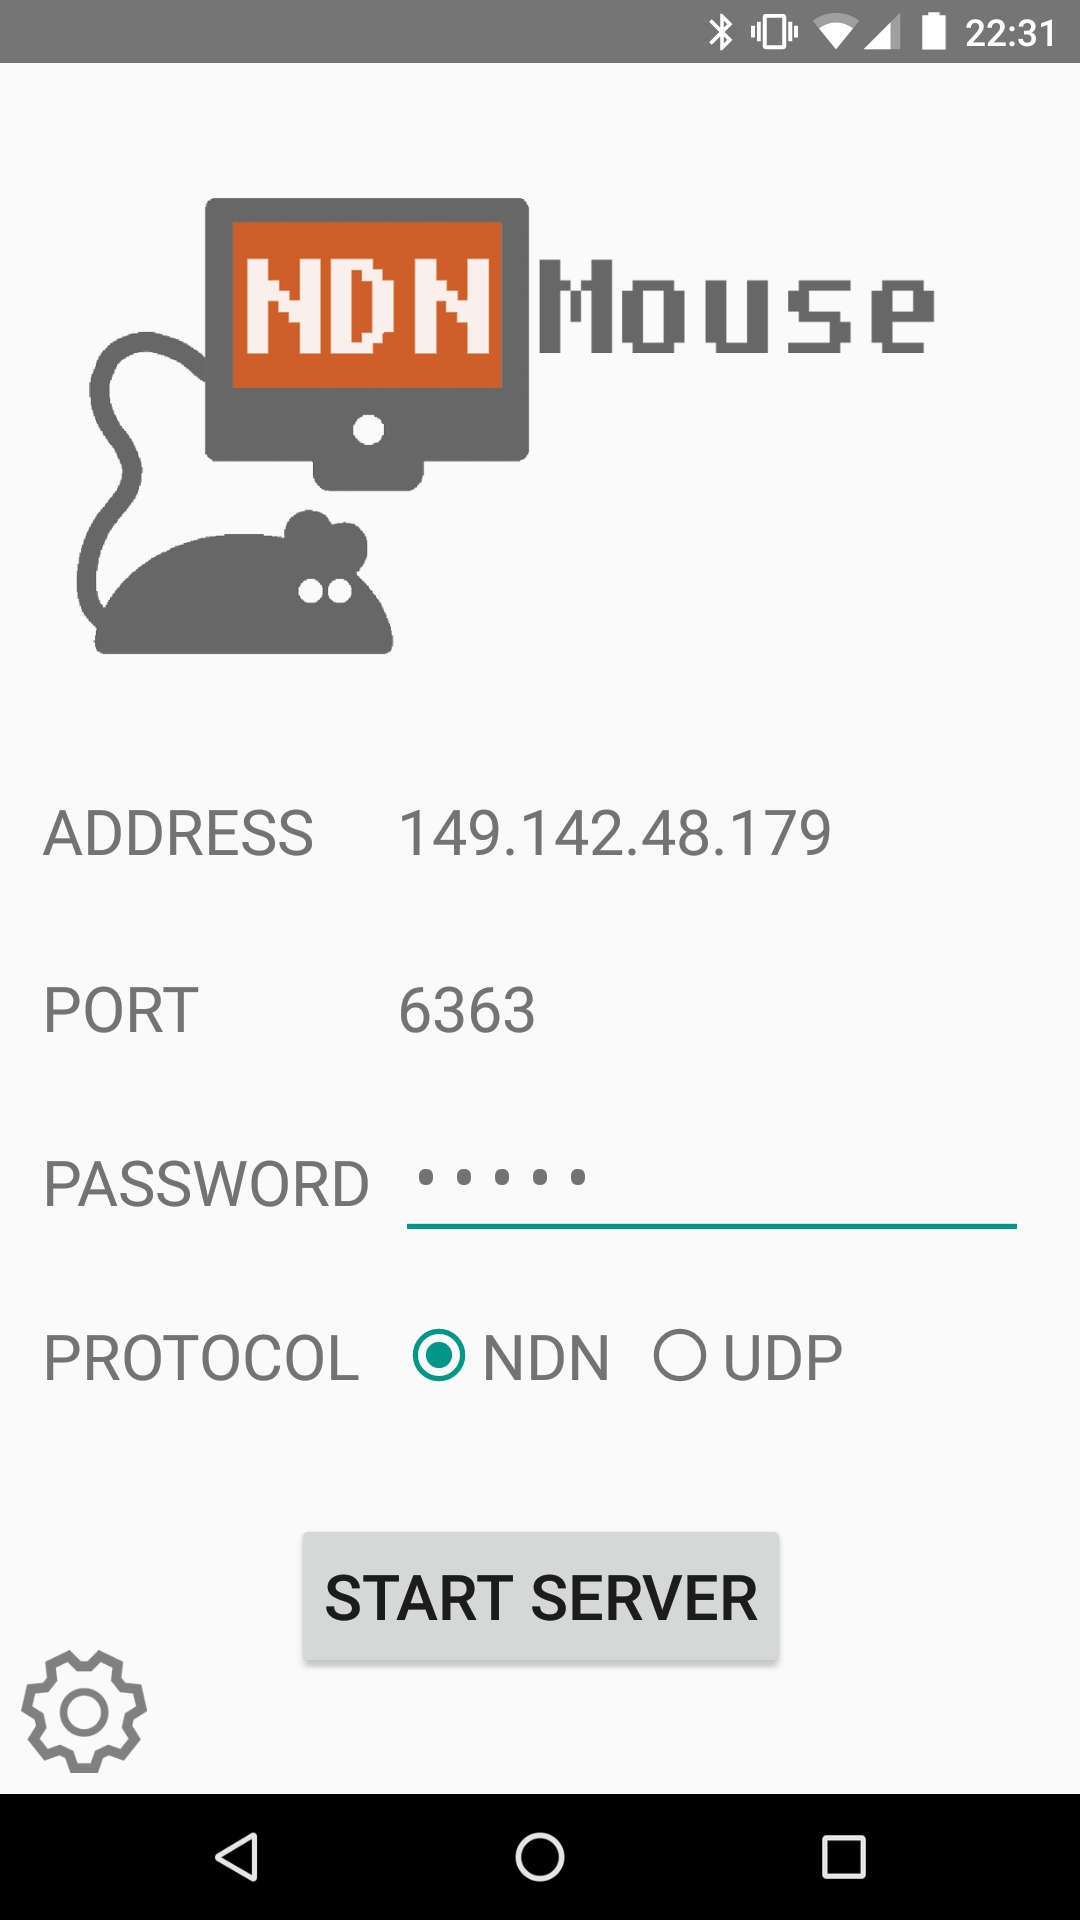
\includegraphics[width=6cm]{screenshots/start}
\end{figure}

\begin{figure}[ht]
	\hypertarget{fig:settings}{}
	\centering
	\caption{Settings screen}
	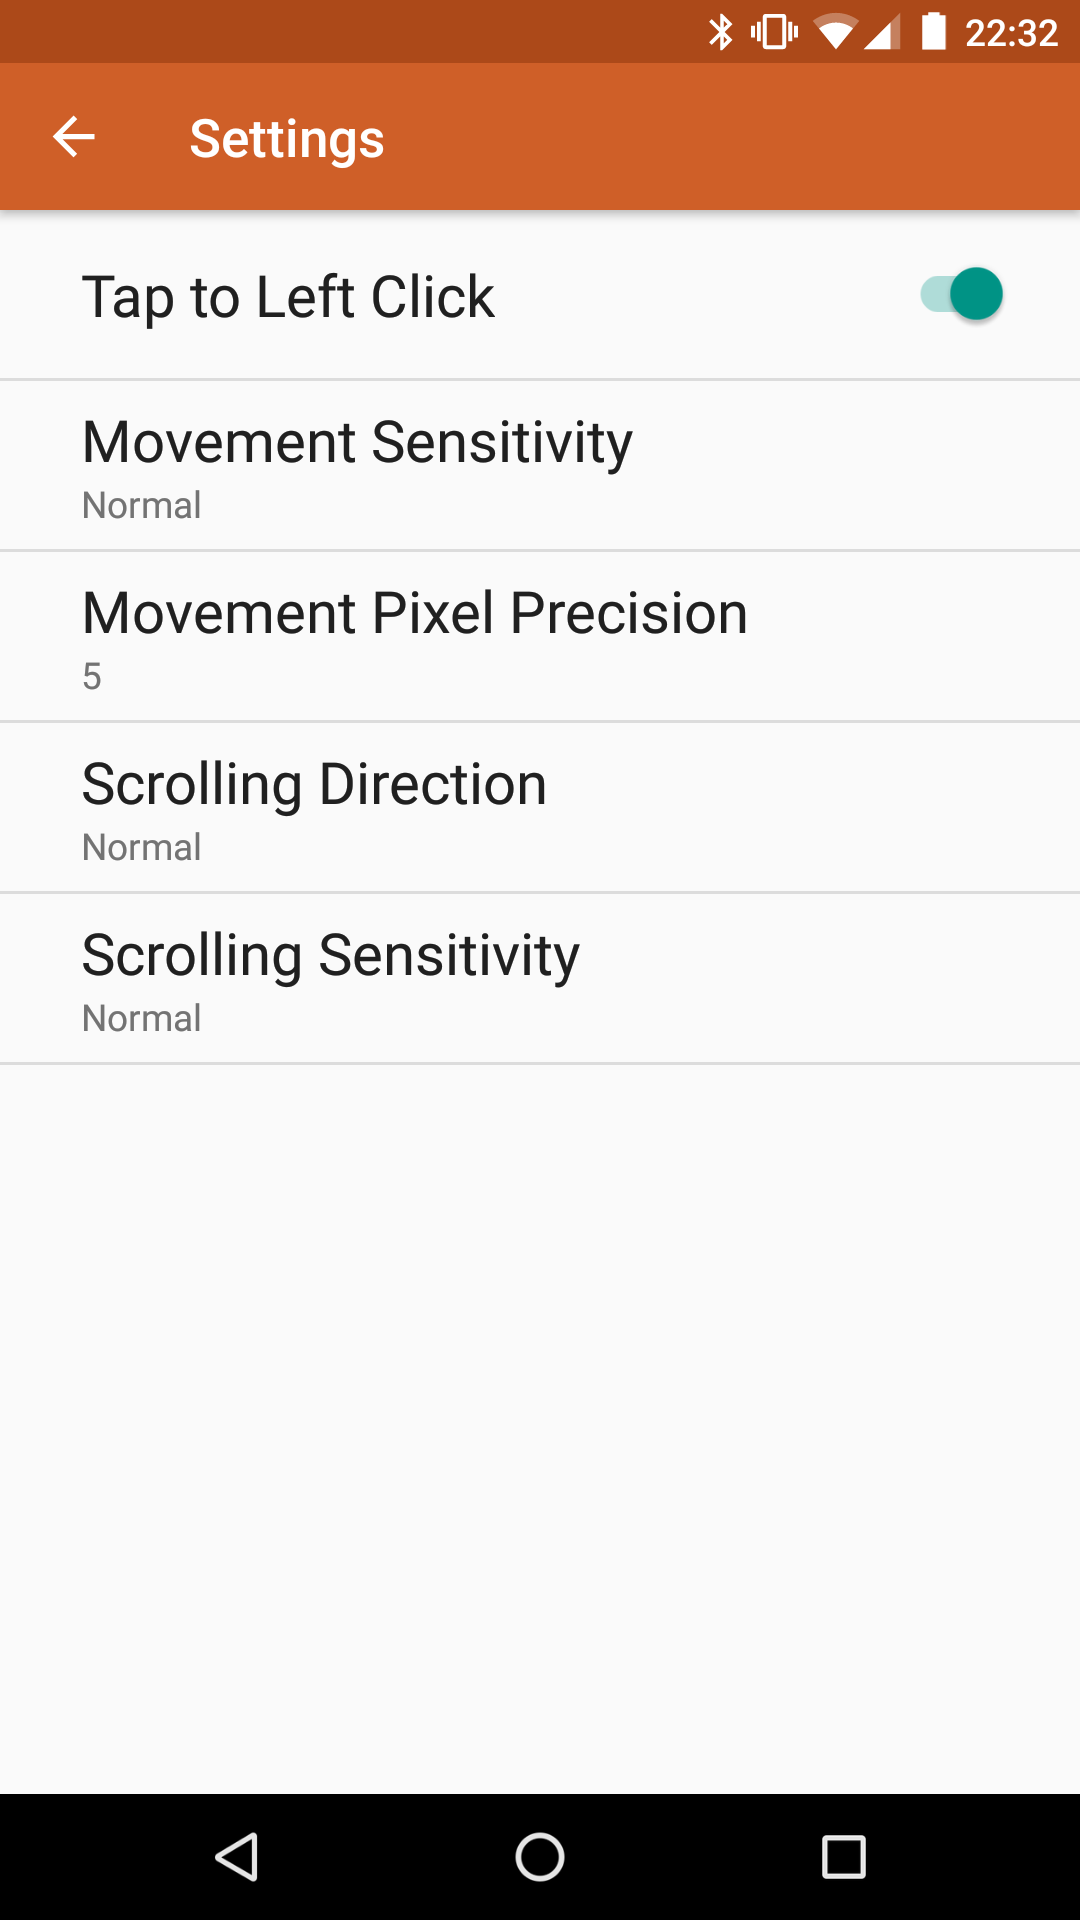
\includegraphics[width=6cm]{screenshots/settings}
\end{figure}

\begin{figure}[ht]
	\hypertarget{fig:touchpad}{}
	\centering
	\caption{Touchpad screen}
	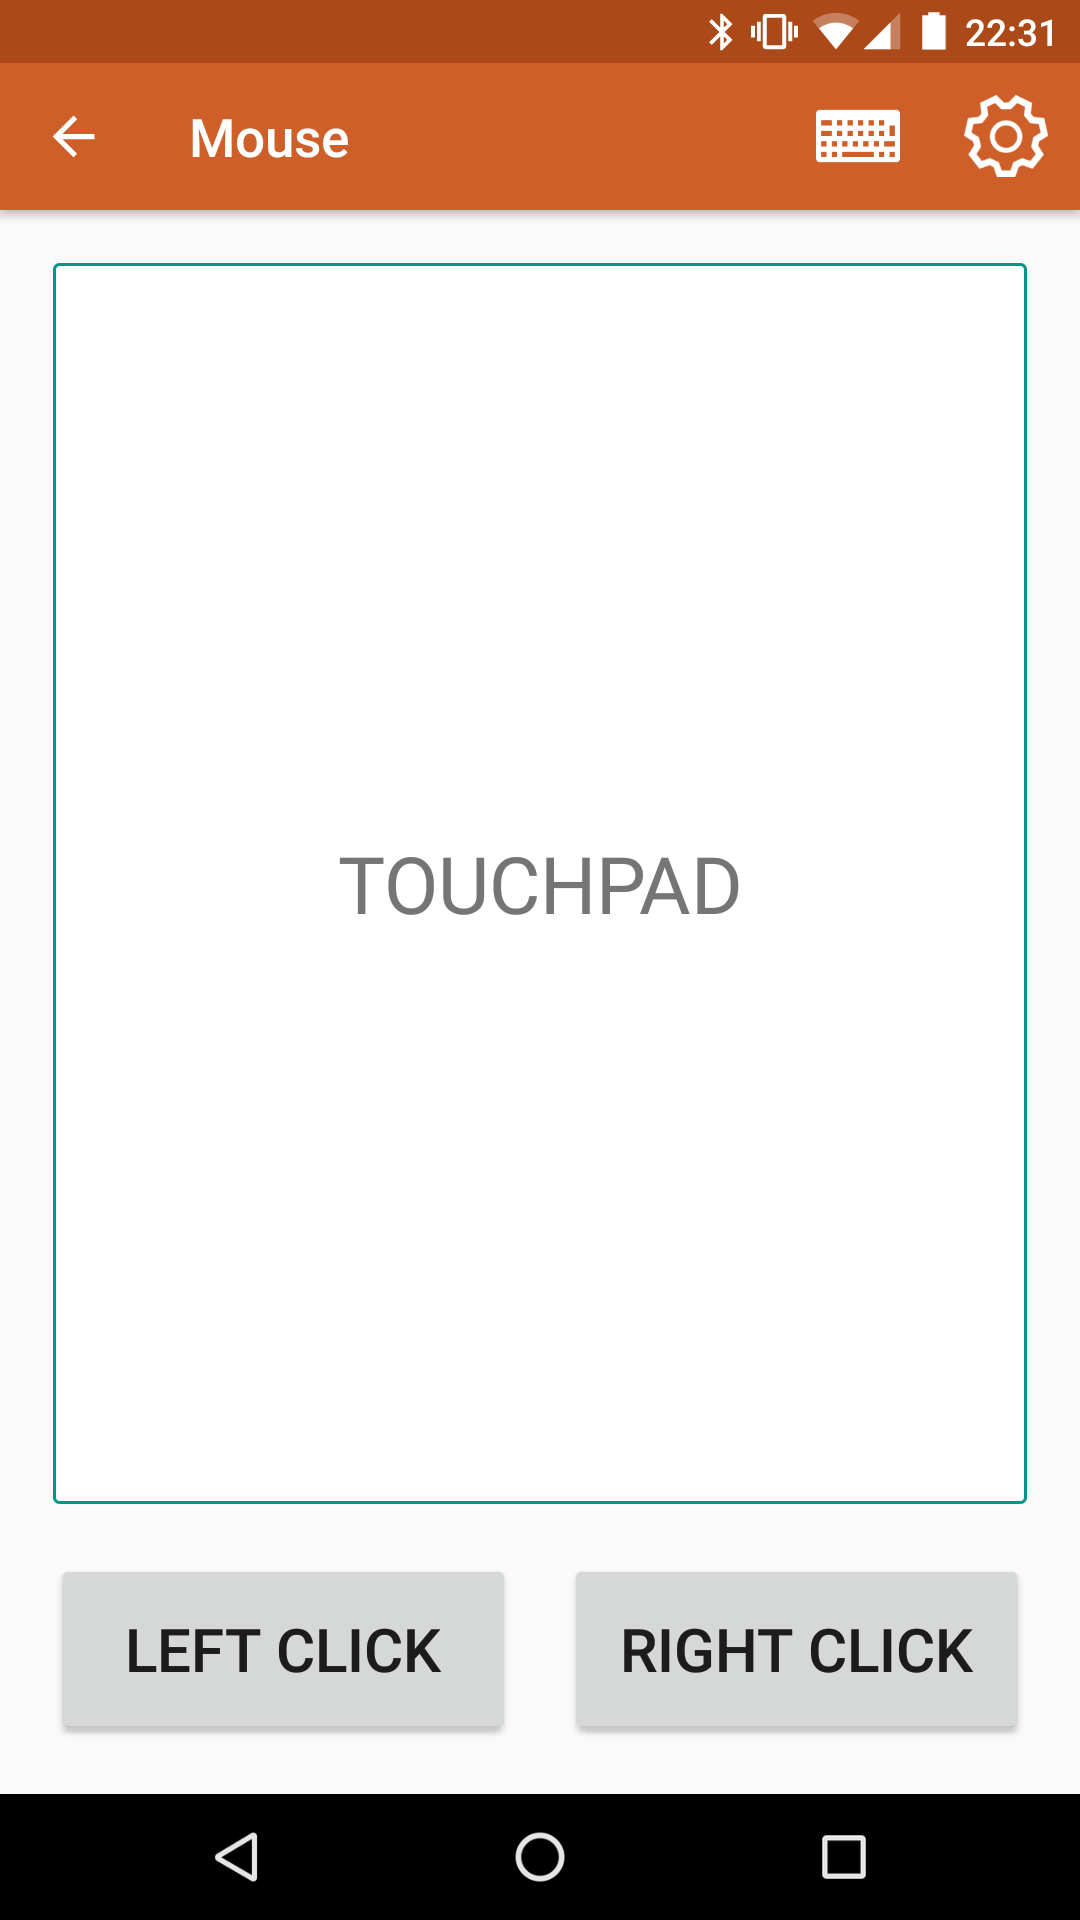
\includegraphics[width=6cm]{screenshots/touchpad}
\end{figure}

\begin{figure}[ht]
	\hypertarget{fig:keyboard}{}
	\centering
	\caption{Keyboard screen}
	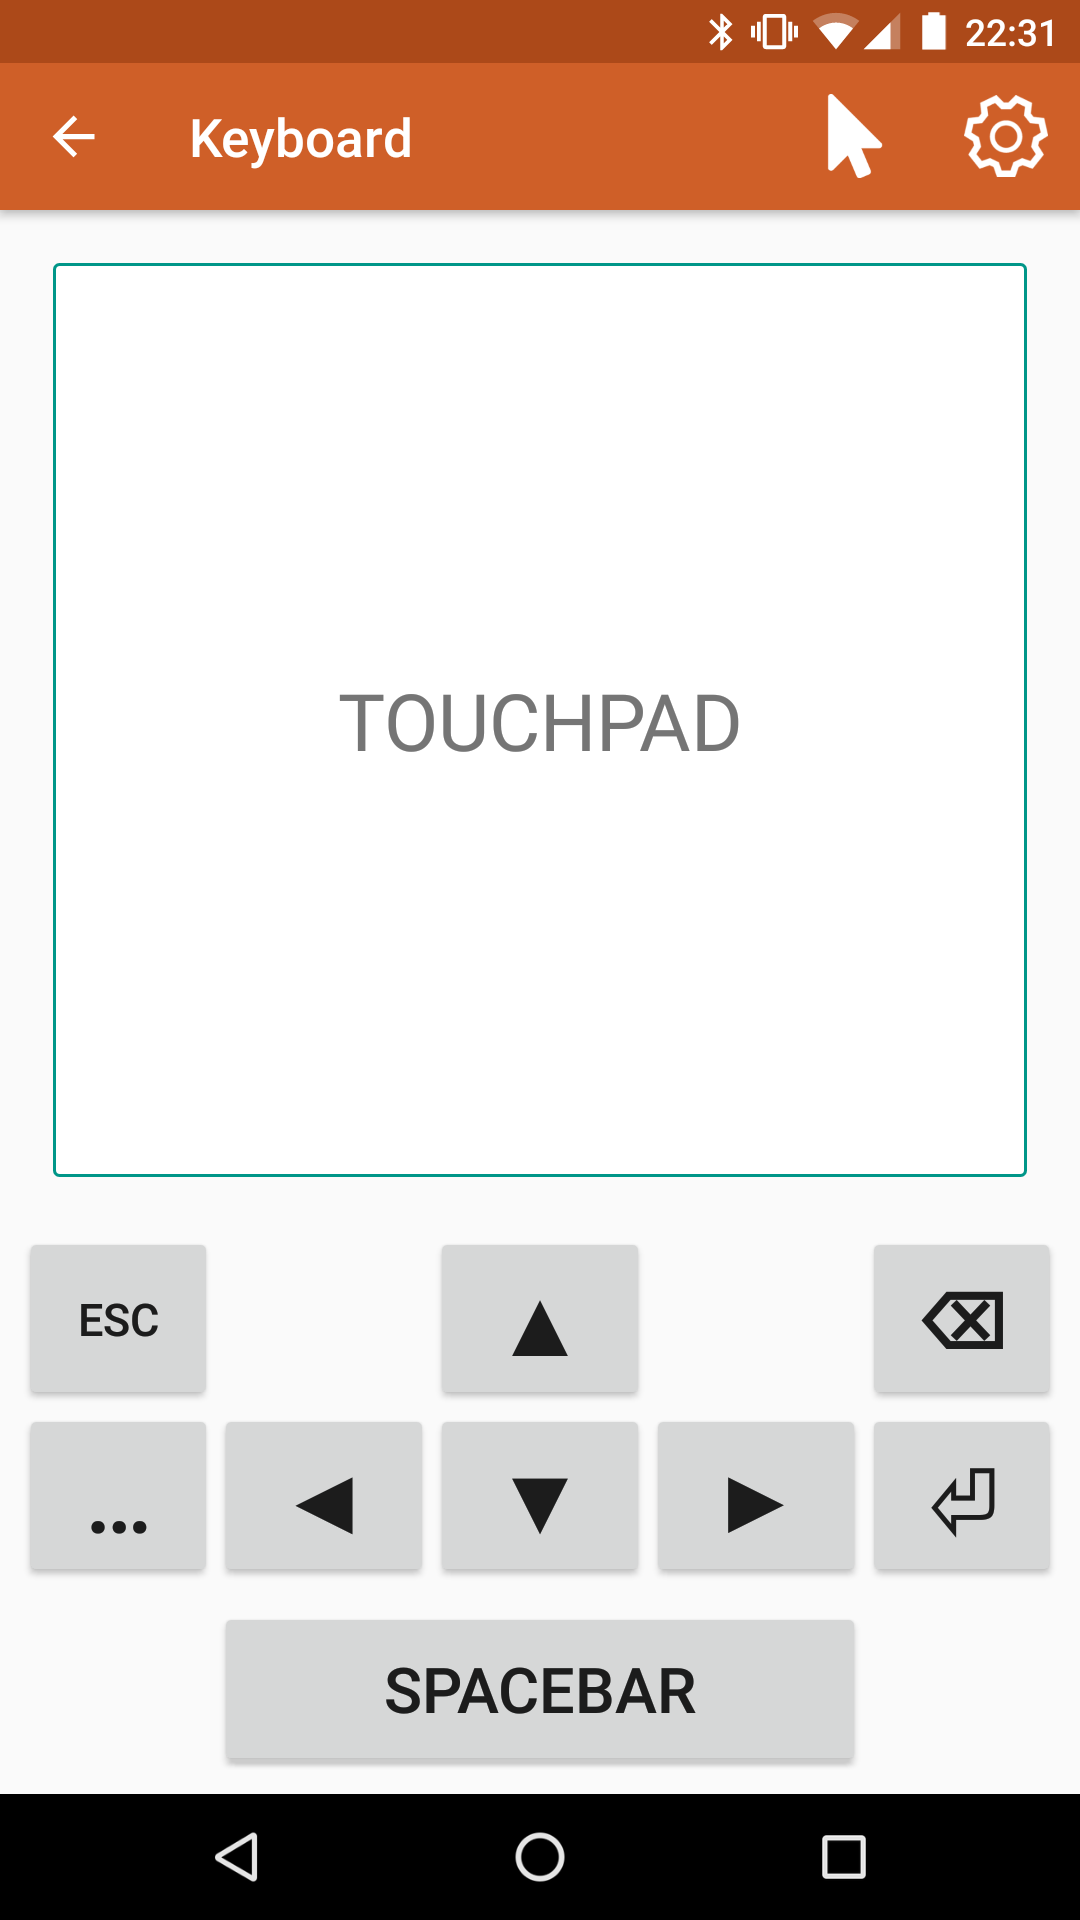
\includegraphics[width=6cm]{screenshots/keyboard}
\end{figure}

\begin{figure}[ht]
	\hypertarget{fig:custom\_type\_message}{}
	\centering
	\caption{Custom typed message entry}
	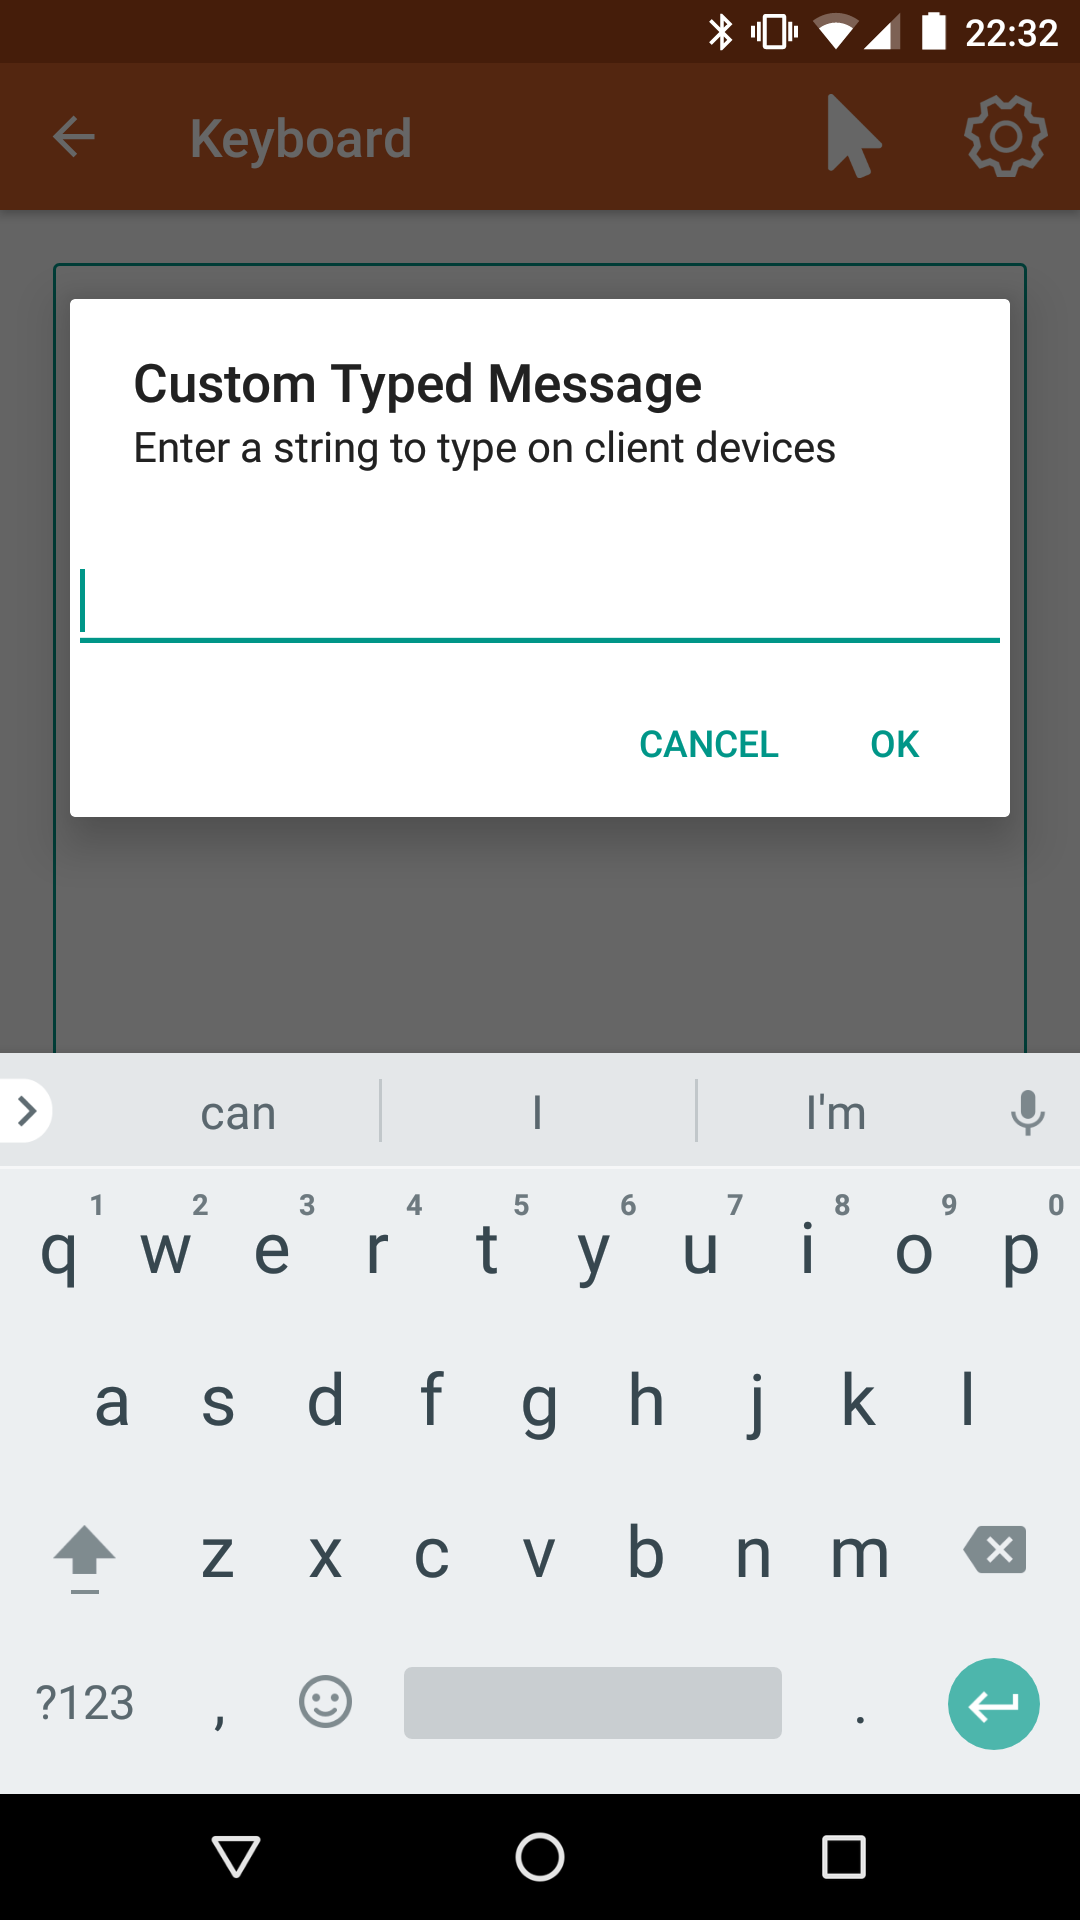
\includegraphics[width=6cm]{screenshots/custom_type_message}
\end{figure}

\begin{figure}[ht]
	\hypertarget{fig:client1}{}
	\centering
	\caption{PC program IP address entry}
	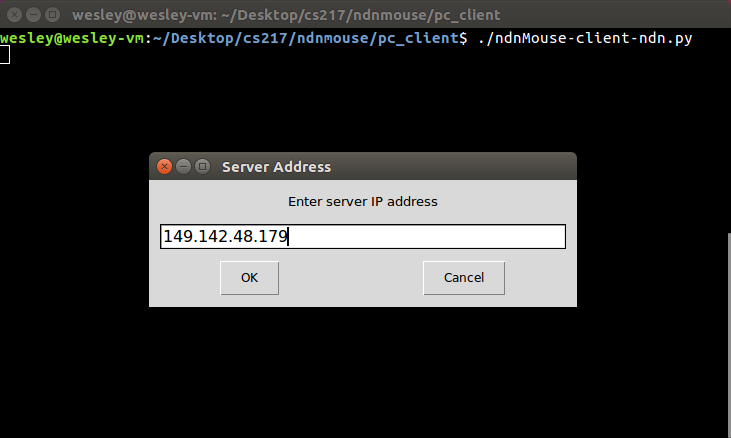
\includegraphics[width=11cm]{screenshots/client1}
\end{figure}

\begin{figure}[ht]
	\hypertarget{fig:client2}{}
	\centering
	\caption{PC program password entry}
	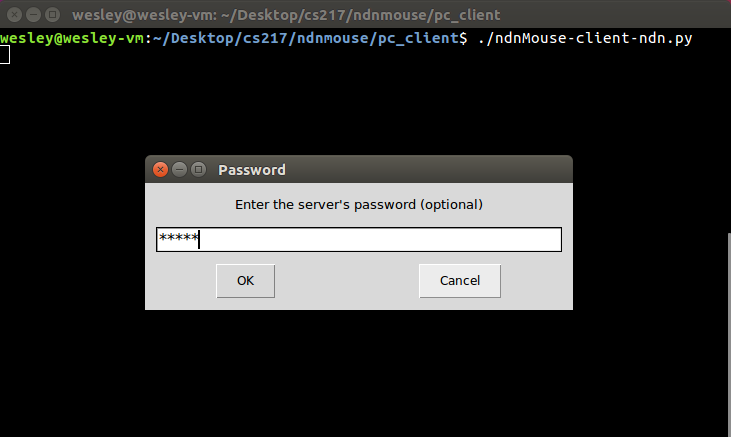
\includegraphics[width=11cm]{screenshots/client2}
\end{figure}

\begin{figure}[ht]
	\hypertarget{fig:client3}{}
	\centering
	\caption{PC program running}
	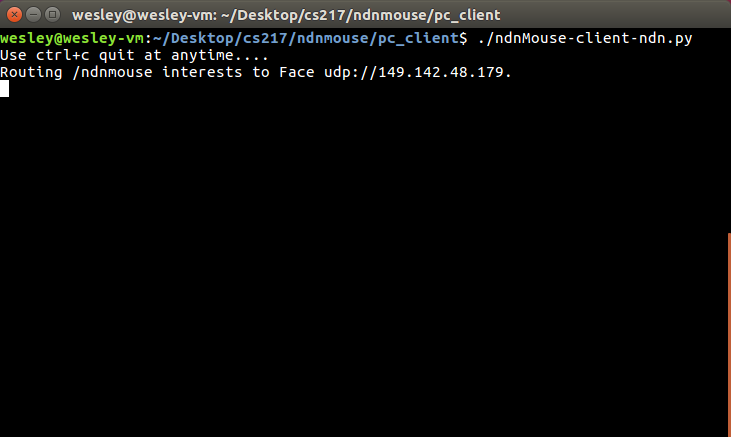
\includegraphics[width=11cm]{screenshots/client3}
\end{figure}

\end{document}